\documentclass[twocolumn]{aastex62}

\newcommand{\vdag}{(v)^\dagger}
\newcommand\aastex{AAS\TeX}
\newcommand\latex{La\TeX}
\usepackage{amsmath}
\usepackage{physics}
\usepackage{hyperref}
\usepackage{natbib}
\usepackage[T1]{fontenc}
\usepackage[english]{babel}
\usepackage[utf8]{inputenc}
\usepackage{wasysym}

\begin{document}

\title{\Large AST5220-Milestone IV: The CMB and Matter Power-Spectra}

\author{Nils-Ole Stutzer}

\begin{abstract}
    We have computed the angular CMB anisotropy and matter power spectrum, as seen today, of the universe simulated by \cite{stutzer:2020a,stutzer:2020b,stutzer:2020c}. The CMB angular power pectrum was found by first computing the multipole moments $\Theta_\ell(k)$, for $0 < \ell \leq 1200$, using a line-of-sight integration by Zaldarriagaand Seljak. The CMB power spectrum was than computed by these multipoles moments as well as the primoridal Harrison-Zel'dovich power spectrum. The integrals were solve using an ODE solver approach and the matter power spectrum was simply computed using the splined quantities from \cite{stutzer:2020c}. The position of the fist peak in the CMB spectrum was found to be at $\ell_* \approx 200$, corresponding to a sound horizon scale at recombination of $k_*\approx 0.02 h/\mathrm{Mpc}$. We found the matter power spectrum to have an onset of Meszaros suppression at the characteristic bend-over set by matter-radiation equality at $k_\text{eq} = 0.015 h/\mathrm{Mpc}$. The resulting spectra behaved according to expectations and were consistent with known physics. In particular, the CMB power spectrum computed matched the one found by \cite{callin:2006} when using the same cosmological parameters.


    \textit{The codes for this paper can be found at:} \newline \url{https://github.com/SagittariusA-Star/AST5220-Milestones}
\end{abstract}

\section{Introduction} \label{sec:Intro}
The aim of cosmology as a science has always been to unearth the secretes of how the Universe was formed and how it has evolved since. As modern high precision
measurements by probes like Planck have shown is how successful the cosmological standard model with dark energy and cold dark matter ($\Lambda$CDM) is in describing the observed data of the CMB and its anisotropies \citep[]{planckcollaboration:2018}. One of the most common ways to estimate the parameter values of the $\Lambda$CDM model infered from the data, is to compare the observed and the theoretical CMB and matter power spectra and find the best-fit by means of a statistical treatment. 

In this paper we will focus on computing the CMB and matter power spectra, by building upon the foundation by \cite{stutzer:2020a}, \cite{stutzer:2020b} and \cite{stutzer:2020c} which computed the background evolution, recombination history and formation of structure from primordial perturbations of the Universe. The ultimate goal of computing the power spectra will be achieved using the same cosmological parameters as \cite{callin:2006}, also previously used in \cite{stutzer:2020a}, \cite{stutzer:2020b} and \cite{stutzer:2020c}. Further more, we will for simplicity neglect the spatial curvature, neutrinos and polarization of photons. 


\section{Method} \label{sec:Method}
When solving for the CMB and matter power spectra in this paper we will mainly use the equations and relations that are provided by \cite{winther:2020c}, \cite{callin:2006} and \cite{dodelson:2003}. Unless otherwise stated the equations presented here are thus provided by these authors and refere the interested reader to them for detailed derivations, and only present the main outline towards computing the power spectra.  


\subsection{The Power Spectra} \label{subsec:spectra}
Before going on to actually computing the power spectra, a few words on what a power spectrum actually is. To find out this we consider the CMB as an example. The CMB as we see it today is build up of an average temperature of $T_\mathrm{CMB} = 2.7255\mathrm{K}$ upon which there are small perturbations of the order $\delta T / T_\mathrm{CMB} \sim 10^{-5}$ seen as anisotropies in the CMB. One can think of the CMB of a function on the celestial sphere that can be expanded in term of its anisotropies of different scales as basis functions. This is done using spherical harmonics as 
\begin{align}
    T(\hat{n}) = \sum_{\ell m} a_{\ell m} Y_{\ell m}(\hat{n}),
\end{align}
where the temperature $T$ in the direction $\hat{n}$ on the sky is given by the sum over the spherical harmonics $Y_{\ell m}$ times the corresponding expansion coefficient $a_{\ell m}$. The indices $\ell$ and $m$ quantify the scale and orientation of the perturbations. For instance $\ell = 0$, $\ell = 1$ and $\ell = 2$ represent the monopole (average temperature), dipole (hot and cold blobs separated by $180^\circ$ on the sky) and the quadrupole (alternating hot and cold separated by $90^\circ$ on the sky).

The angular power spectrum of the CMB anisotropies is simply related to this expansion and corresponds to the expected value of the expansion coefficient squared for each scale $\ell$
\begin{align}
    C_\ell = \langle |a_{\ell m}|^2 \rangle = \langle a_{\ell m}a_{\ell m}^* \rangle.
\end{align}
In principle, though, there should be a dependence on the orientation $m$, however, since the CMB according to the underlying cosmological principle must be isotropic on large scales we can simply average out the directional dependence without large errors. The angular power spectrum $C_\ell$ hence quantifies how much contribution to the CMB there is on each angular scale, i.e. the amplitude, and can be understood as a correlation function between to points of a given angular separation. 

In order to compute the power spectrum $C_\ell$ we need the coefficients $a_{\ell m}$ which are given by the temperature field at time $x = \ln a(t)$ $T(\hat{n}, x)$. The temperature fields evolution through time $x$ and for different scales $k$ were found in \cite{stutzer:2020c} in the form of the photon perturbation multipole moments $\Theta_\ell(k, x)$. These multipole moments were however found in fourier $\vec{k}$-space, but we want to have them in real ($\vec{n}$-) space at the present time. To get the perturbations $\Theta_\ell(\hat{n}, x)$ today, we simply inverse fourier transform and evaluate the result at the present time $x = 0$. 

There is only one caveat to this idea. In order to compute all the coefficients $a_{\ell m}$ we would need the infinite series of multipole monents $\Theta_\ell$, however, \cite{stutzer:2020c} only computed around 8 of them, but we would need around $\ell_text{max} \sim 1200$ to get a decent power spectrum \citep[]{winther:2020c}. Solving for all the multipole moments up to $\ell = 1200$ using the approach of \cite{stutzer:2020c} would take a long time and be very inefficient. 

Fortunately Zaldarriaga and Seljak solved this problem for us by inventing the \textit{line-of-sight} integration. To obtain the coupled equations for the$ \Theta_\ell$'s in the first place one used the photon perturbation $\Theta(k, \mu, x)$, being a function of angle $\mu = \cos \theta$. Thus one can, instead expanding the perturbation equation into multipoles and then solving the long coupled system of differential equations as in \cite{stutzer:2020c} (but with $\ell_\text{max} = 1200$), integrate up the equation for the underlying $\dot{\Theta}$ subsequently find the multipoles. This is shown in detail by \cite{callin:2006} and \cite{dodelson:2003} and yields the following integral for the multipoles 
\begin{align}
    \Theta_\ell(k, x=0) = \int_{-\infty}^{0} \tilde{S}(k,x)
              j_\ell[k(\eta_0-\eta)] dx,
    \label{eq:transfer}
\end{align} 
where $j_ll$ are the spherical Bessel functions being highly oscillatory functions function as an orthogonal basis here that basically project the project the 3D spatial temperature field onto the 2D celestial sphere (as we observe it) and $\eta$ (subscript 0) is the conformal time (today). The multipole index $\ell$ roughly represents the scale of a perturbation, and the mapping between index and scale is roughly $\ell\sim k\eta_0$. The $Theta_\ell(k, x = 0)$ is also called the transfer function and quantifies the multipole moments of the photons for each scale.

The quantity $\tilde{S}(k,x)$ is called the source function and is given by
\begin{align}
    \tilde{S}(x, k) &= \tilde{g}\left[ \Theta_0 + \Psi + \frac{1}{4}\Pi\right] + e^{-\tau} \left[\Psi^\prime-\Phi^\prime\right] \nonumber\\
    &- \frac{1}{ck}\frac{d}{dx}(\mathcal{H}\tilde{g}v_b) + \frac{3}{4c^2k^2} \frac{d}{dx} \left[\mathcal{H}\frac{d}{dx} (\mathcal{H}\tilde{g}\Pi)\right],
    \label{eq:source}
\end{align}
where the metric potential perturbations $\Psi$ and $\Phi$, the baryon velocity $v_b$ and the photon mono- and quadrupole $\Theta_0$ and $\Theta_2$ ($\Pi = \Theta_2$ if polarization is neglected) are all computed by \cite{stutzer:2020c}. The optical depth $\tau$ and visibility function $\tilde{g}$, and the reduced Hubble parameter $\mathcal{H}$ are found by \cite{stutzer:2020b} and \cite{stutzer:2020a} respectively. The source function quantifies how light is affected (both extinction and emission) when traveling through a medium, which in our case is the universe.

This approach of finding the multipoles $Theta_\ell$ is much faster as we only need $Theta_0$ and $\Theta_2$ from the coupled set of ODEs and it has the advantage of being easier to understand. Intuitively one can interpret the line-of-sight integration as integrating up a local radiation monopole through the universes history, which is represented by the term $\tilde{g}\Theta_0$. The terms $tilde{g}\Psi$ and $\tilde{g}\frac{1}{4}\Pi$ are corrections from the photons loosing energy through the potential wells and the correction of the local quadrupole (polarization if included) respectively. Secondly one can spot how the radiation field is affected by the change of the gravitational potentials, seen in the second part of $\tilde{S}$, and represents the gain in energy through the so-called Integrated Sachs-Wolf (ISW) effect. Basically the ISW is that photons that fall into a potential well will gain energy, but lose less than they gained when exiting, since the gravitational wells have decayed due to spatial expansion while the photon traveled through it. The third part of $\tilde{S}$ is simply a doppler effect term.

Now that we have all the $\Theta_\ell$'s we can finally find the power spectrum $C_\ell$. As computed by \cite{stutzer:2020c} the metric perturbations are initially of order $\Psi \sim 1$ which was the underlying initial condition for the whole set of coupled equations for the perturbations. To get the actual initially condition set up by inflation the multipoles (squared) are simply multiplied by the primordial power spectrum, given by the Harrison-Zel'dovich spectrum $P_\text{primordial}(k)$ given by
\begin{align}
    \frac{k^3}{2\pi^2} P_{\rm primordial}(k) = A_s \left(\frac{k}{k_{\rm pivot}}\right)^{n_s-1}.\label{eq:primpow}
\end{align}
The primordial amplitude parameter $A_s \sim 2\cdot 10^{-9}$ at a pivot scale $k_{\rm pivot} = 0.05/$Mpc and the spectral index of scalar perturbations $n_s \approx 0.96$. The primordial amplitude thus quantifies the overall hight of the spectrum, while the spectral index and the pivot scale quantify the tilt and whether the primordial spectrum is scale invariant (which is not since $n_s \neq 1$). 
This simple rescaling we can simply do since all equations are linear. The final power spectrum is then simply found by integrating up all the squared multipoles weighted by $P_\text{primordial}(k)$ over all of $\vec{k}$-space
\begin{align}
    C_\ell &= C_\ell = \frac{2}{\pi}\int k^2P_{\rm primordial}(k) \Theta_\ell^2(k)dk\\
    & =  4\pi \int_0^{\infty} A_s \left(\frac{k}{k_{\rm pivot}}\right)^{n_s-1} \Theta_\ell^2(k) \frac{dk}{k},
\end{align}
where we could simply transform the 3D integral to a 1D integral because of isotropy.
It is common to present the CMB angular power spectrum $\frac{\ell(\ell + 1)}{2\pi}C_\ell$ in units $\mathrm{\mu K^2}$, which is obtained by multiplying it with $(10^6T_\mathrm{CMB})^2$. The prefactor $\frac{\ell(\ell + 1)}{2\pi}$ is used for cosmetic purpose, to eliminate some of the tilt of the spectrum.

The next thing to compute is the matter (both dark and baryonic) power spectrum. This turns out, is the easiest part of the work in this paper, as it is simply found by things we already know from \cite{stutzer:2020c}.
\begin{align}
    P_M(k,x) = |\Delta_M(k,x)|^2P_{\rm primordial}(k),
\end{align} 
where the comoving density contrast $\Delta_M(k, x)$ (which is gauge invariant) is given by 
\begin{align}
    \Delta_M(k,x) \equiv \frac{c^2k^2\Phi(k,x)}{\frac{3}{2}\Omega_{M 0} a^{-1} H_0^2}\label{eq:DeltaM}
\end{align}
\citep[]{winther:2020c}. This we can simply compute at the present time $x = 0$ by using the splined quantities from \cite{stutzer:2020c} that go into \ref{eq:DeltaM}. 

The power spectra for the CMB $C_\ell$ and for matter $P_M(k)$ are then plotted versus multipole index $\ell$ and (comoving) wavenumber $k$.



\subsection{The Implementation} \label{subsec:implementation}
When it comes to the implementation of the above mentioned methodology most things are fairly strait forward. All the perturbation multipole moments as well as the background and recombination quantities are found by \cite{stutzer:2020c}, \cite{stutzer:2020b} and \cite{stutzer:2020a} respectively. These are then used to evaluate and save $\tilde{S}(x, k)$ over a $x,k$-grid, which subsequently is splined using the \texttt{Spline2D}-routine by \cite{winther:2020b} to make a more continuous callable representation. 

Next to solve the first integral for the transfer function, i.e. eq. (\ref{eq:transfer}), we can choose several approaches; either one could use some numerical integration routine or one could solve the integral as an ODE
\begin{align}
    \dv{\Theta_ell}{x}(k, x = 0) = \tilde{S}(k,x)
    j_\ell[k(\eta_0-\eta)].\label{eq:ode1}
\end{align}
Both have advantages and disadvantages, the first being the safest as the numerical integration minimizes the global error, while solving an ODE one can only really manage the local error. Basically it boils down to extrapolation being "riskier" than interpolation. However, the main advantage with solving the integral as an ODE is that we could use the already sat up infra structure by \cite{stutzer:2020a,stutzer:2020b,stutzer:2020c}. Since we already have the means to solve the integrals this way we chose the ODE approach, which should work just fine as longe as we are careful with the grid resolution and tweak the allowed relative local errors, and since the integrands we consider are fairly well behaved. Hence the main structure of the algorithm is to loop through the different multipole indices $\ell$, and solve integral using the \texttt{ODEsolver}-routine by \cite{winther:2020a}, subsequently saving the result. The initial condition for the ODE (\ref{eq:ode1}) is simply $\Theta_\ell(k, -\infty) = 0$, which we can see from the $Theta_\ell$'s in \cite{stutzer:2020c} as the perturbations stay zero outside the horizon. The next integral is solved the exact same way with the ODE
\begin{align}
    \dv{C_\ell}{\ln k} = 4\pi A_s \left(\frac{k}{k_{\rm pivot}}\right)^{n_s-1} \Theta_\ell^2(k),
\end{align}
just using the \texttt{ODEsolver}-routine by \cite{winther:2020a} and initial conditions $C_\ell(k = 0) = 0$. Now, using this initial condition might introduce a small error, since $C_\ell(k = 0)$ does not strictly equal zero, but the error is really small and hence negligible. The obtained values for all the $C_\ell$'s are then splined using the \texttt{Spline}-routine by \cite{winther:2020a}. 

When computing the fist integral we used the C++ (17) standard library spherical Bessel functions. However, we run into some problems evaluating these for higher $\ell$, as the standard library Bessel functions returned \texttt{NaN} at some points where the function should be basically zero. Thus when making splines of the $j_\ell$'s we only included indices up to $\ell_\text{max} = 1200$ and we included an approximation ensuring the value of $j_\ell = 0$ (as they should) at the critical points. 

Then when computing the matter power spectrum, we don't need to make any splines since we already have all the needed functions and splines of their components (in particular we have the spline of $\Phi(k, x)$ from \cite{stutzer:2020c}), wo we just make a callable function straight away. 

The power spectra (, the transfer function $\Theta_\ell(k, x = 0)$ and the integrant $\Theta_\ell^2 / k$) are than evaluated and saved to files for plotting in Python.

\begin{figure*}
    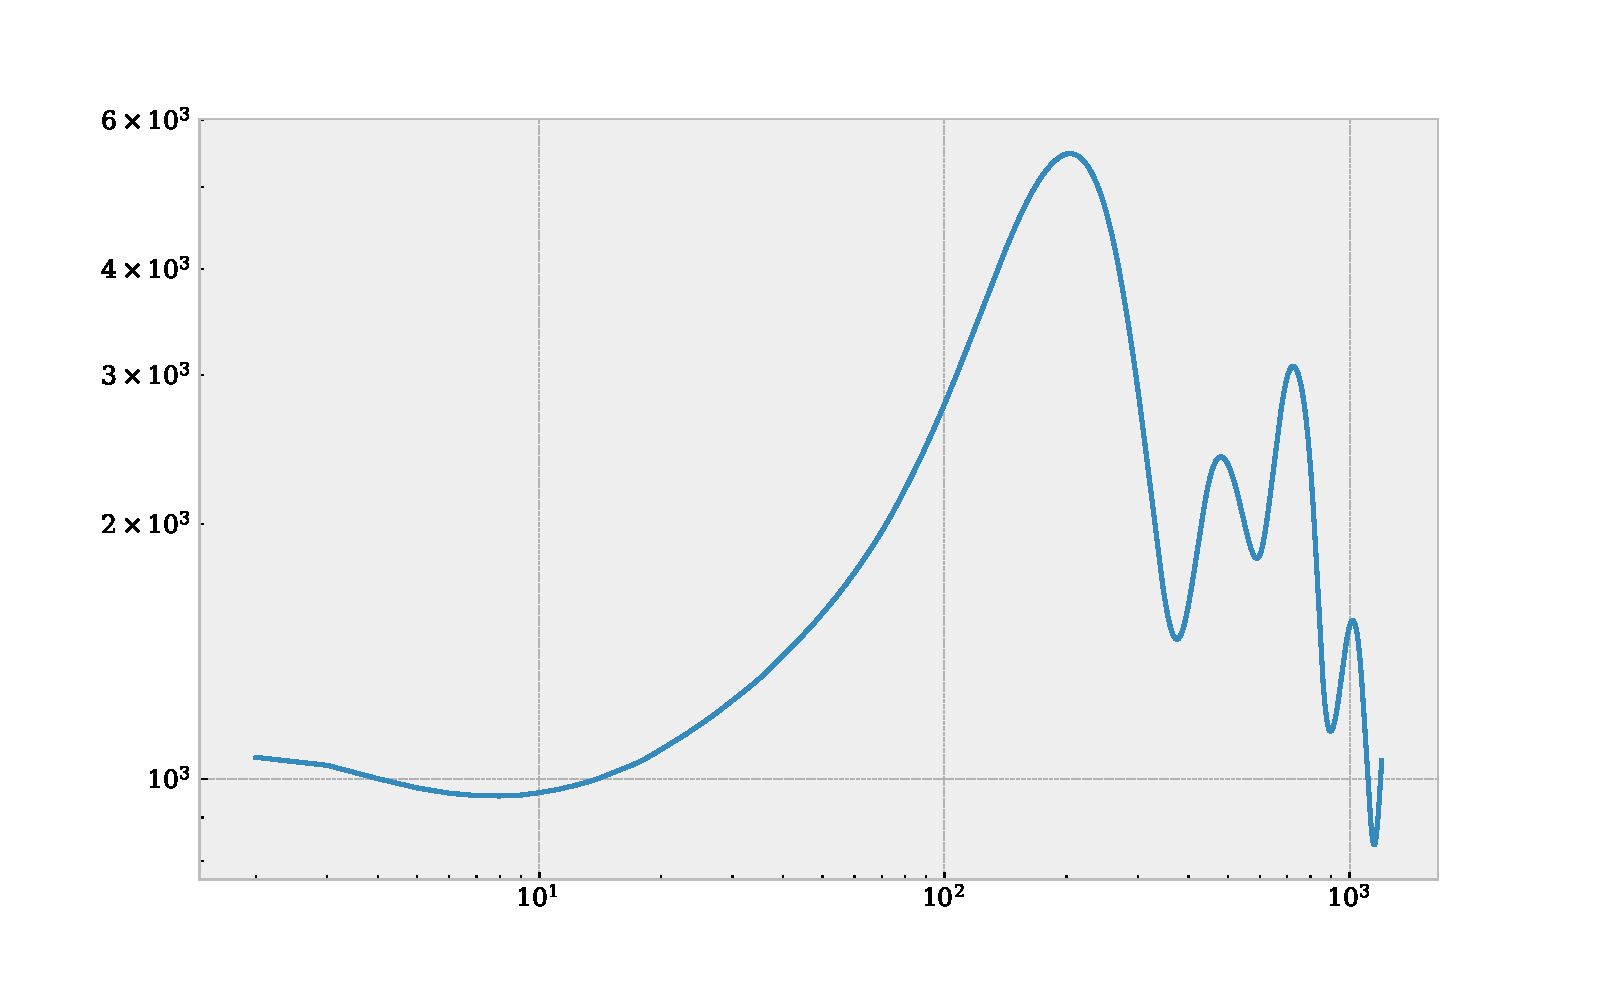
\includegraphics[scale = 0.65]{Figures/Cell.pdf}
    \caption{\textbf{Upper panel}: The figure shows the CMB angular power spectrum for different scales given by the multipole index $\ell$, for $0 < \ell < \ell_\text{max} = 1200$, in units $\mathrm{\mu K}^2$, as seen today for the cosmological parameters also used by \cite{stutzer:2020a,stutzer:2020b,stutzer:2020c}. The peaks and troughs are indicated as solid and dashed lines respectively.\textbf{Middle panel}: The figure is showing two additional power spectra to the one in the upper panel, with different baryon-to-CDM ratios as marked in the legend.  \textbf{Lower panel}: The figure shows the matter power spectrum as a function of the comoving wavenumber $k$, as seen today. The scale $k_\text{eq} = 0.015 \mathrm{h / Mpc}$ of the horizon at matter-radiation equality is marked by a dashed red line.} 
    \label{fig:Cell}
\end{figure*}

\begin{figure*}
    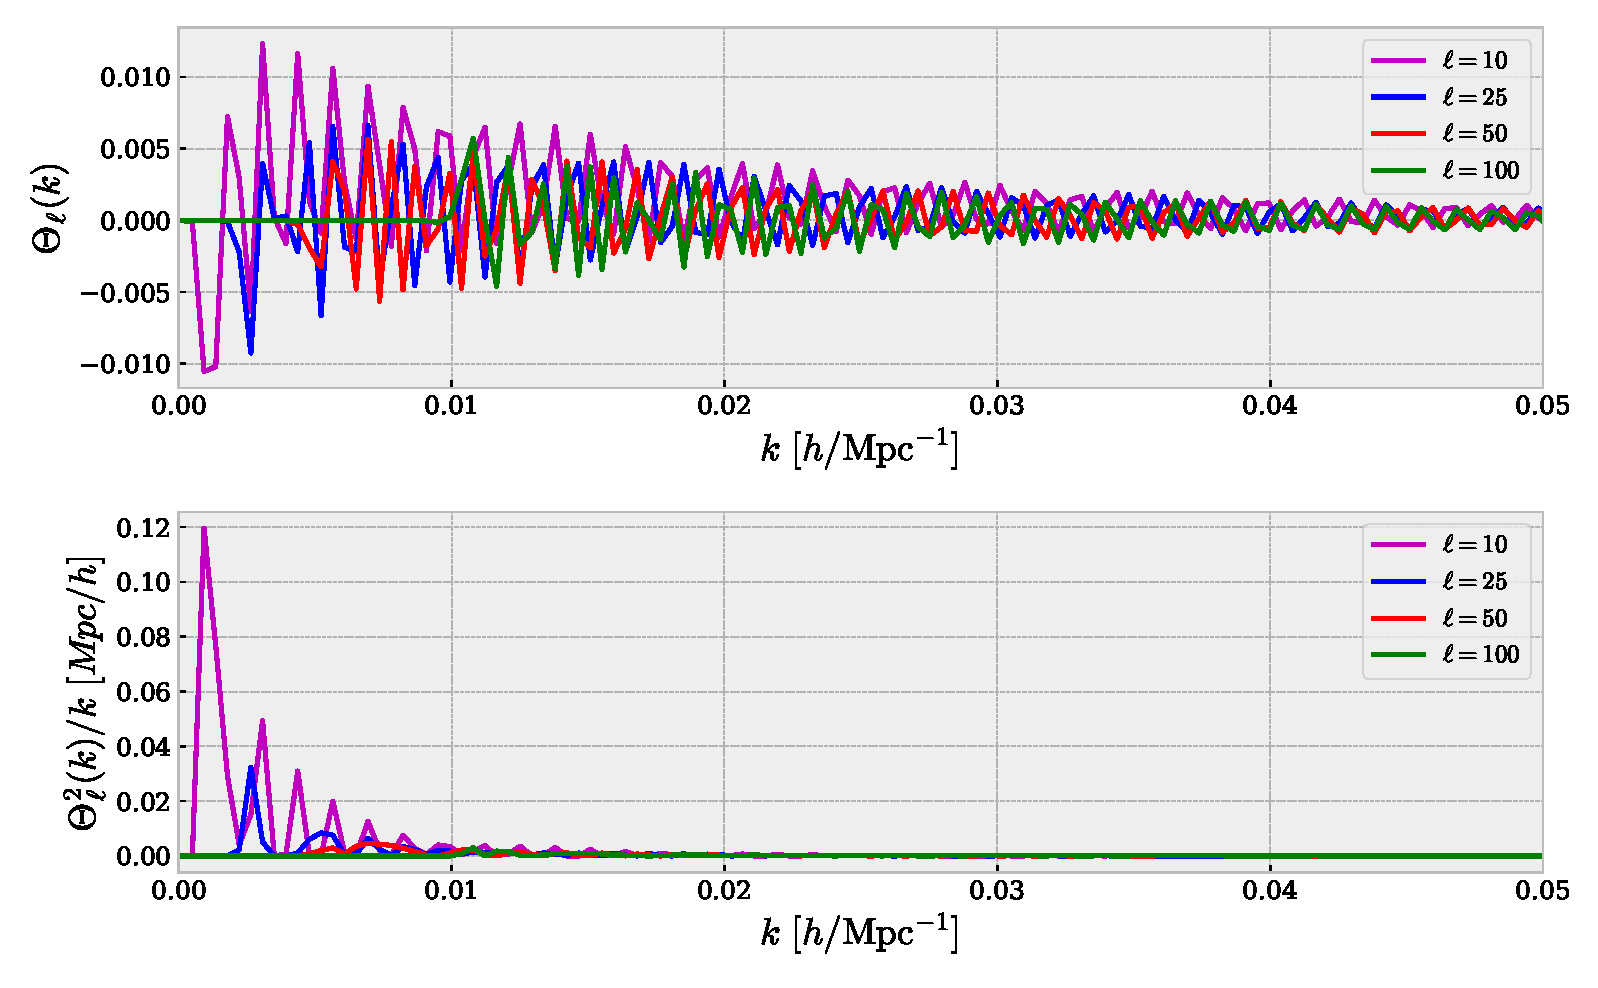
\includegraphics[scale = 0.65]{Figures/Transfer_func.pdf}
    \caption{\textbf{Upper panel}: The figure shows the radiation transfer functions $\Theta_\ell(k)$ as a function of comoving wavenumber $k$, for the multipoles $\ell = 10, 25, 50$ and $100$. \textbf{Lower panel}: The figure shows the integrand to the power spectrum (expept the primordial power spectrum bit) as a function of comoving wave number, for the multipoles $\ell = 10, 25, 50$ and $100$.}
    \label{fig:Transfer_func}
\end{figure*}

\section{Results / Discussion}\label{sec:Results/Discussion}
The results from our computations can be seen in Figure \ref{fig:Cell} and \ref{fig:Transfer_func}. Figure \ref{fig:Cell} shows both the CMB and the matter power spectrum as seen today. 

We first consider the CMB power spectrum as seen in the upper panel of Figure \ref{fig:Cell}. The CMB power spectrum illustrate how different scaled (local monopole, i.e. overdensities) perturbations were frozen in as the universe became transparent at the last-scattering surface of recombination. Thus the $C_\ell$ can be interpreted as the contribution of a scale $l\sim k\eta_0$ to the CMB. The first thing one can notice is that on the largest scales, i.e. smallest $\ell$, we see a plato with a slight but noticeable negative tilt. At these large scales which are superhorizon scales until recently remain relatively unchanged throughout their evolution from the time of recombination till today, and will stay as they were set up by inflation initially, as seen in \cite{stutzer:2020c}. The initial conditions set up by inflation are as mentioned in Sec. \ref{subsec:spectra} given by the primordial power spectrum in eq. (\ref{eq:primpow}). Thus as the perturbations, i.e. the transfer functions eq. (\ref{eq:transfer}) are essentially constants for large scales, the plato represents the primordial power spectrum itself. Since $n_s =0.96$, slightly less than unity, we expect the observed slight negative tilt away from scale invariance. Further more we see the CMB power spectrum for low multipoles having a non-zero contribution, which is due to the primordial amplitude $A_s$ being non-zero.

The next thing we consider are the characteristic peak and trough pattern in the CMB power spectrum. These are the imprint of the acoustic oscillations also observed in \cite{stutzer:2020c}. As discussed in \cite{stutzer:2020c}, the peaks and troughs are the contribution of the perturbations that performed half or full number of oscillations, i.e. had an extrema or a zeros at recombination, respectively by the time of recombination $x_*$. Thus the $\ell$ of the fist peak $\ell_*\sim 200$ will approximately represent the scale of the sound horizon at recombination. Using the relation $k \sim \ell / \eta_0 \approx 0.02 h/\mathrm{Mpc}$ using the value of $\eta_0$ from \cite{stutzer:2020a}. This scale is important since it can be used as a standard ruler when measuring cosmological distances. 

Nevertheless, there are more interesting details to note in the acoustic peaks. The fist of them being that the fist acoustic peak is quite tall compared to the others. This is the imprint of the ISW effect. The ISW effect can as mentioned be understood by looking at the second part of eq. (\ref{eq:source}) containing the derivatives of the metric potentials. As can be seen in \cite{stutzer:2020c} the metric potentials will start to decay once they enter the horizon prior to matter-radiation equality, and continue decaying until crossing into matter dominance. Now, the potential perturbations that contribution the most to the ISW effect are those that have the largest derivatives of the potentials at the time of recombination (which is discussed in greater detail in \cite{dodelson:2003}), which as we can see from Figure 1 in \cite{stutzer:2020c} corresponds about to the scale of the first acoustic peak in the CMB power spectrum. The transfer functions in eq. (\ref{eq:transfer}) are thus boosted by the potential decay at this scale, resulting in the first peak being taller than the others, which correspond to scales were the potentials have a more constant shape at recombination.

Next we can notice that every second peak in the CMB power spectrum seems to be taller than the one before. This is a consequence of the ballance of dark matter and baryons in the power spectrum. When considering a cosmology with almost all matter being cold dark, having very little baryons, this is what we will observe. If baryons would dominate the dark matter content, we would not see this alternating hight, but rather that each peak is taller than the subsequent one. So by the hight relation between the peaks one can estimate the ratio of baryonic and dark matter content of the universe. The behaviour of $C_\ell$ when changing the baryon-to-CDM ratio is illustrated in the middle panel of Figure \ref{fig:Cell}, where we have overplotted the CMB power spectrum of two additional cosmologies, one with more baryons than CDM and vice versa (see legend). In general the CMB power spectrum is very sensitive to cosmological parameter, and can thus be used for a parameter estimate of data measured by a probe, we however have only shown the dependence of the matter density parameters as an example here, but other parameters can cause analogous changes to the spectrum.

Next, we note the so-called dampening tail of the CMB power spectrum. Unfortunately, due to the \texttt{NaN} problems of the C++ standard library spherical Bessel functions, we could not compute higher $C_\ell$'s than $\ell_\text{max} \sim 1200$. The dampening tail is thus unfortunately not seen as nice as we had hoped. However, one can still see that the hight of the peaks, and the acoustic oscillation pattern in general, seem to decreases in hight and that the power spectrum as whole decreases at higher $\ell$. The reason this happens for the higher multipoles is simply diffusion. At small scales early on there are non-negligible contributions from the local quadrupole; hot photons are diffusing into the cold regions nearby, and vice versa. Since the medium was hot and dense before recombination and photons scattered often, the mean-free-path and hence the diffusion length was small, making only small scales able to be affected by the smoothing of diffusion. Therefore, we see that for increasing multipoles $\ell$, i.e. decreasing scale that the contribution to the CMB power decreases, while large scales are left unaffected.

There are probably even more interesting details in the CMB power specter we present, however, we have now presented the most important and the most noticeable features and thus continue to the matter power spectrum seen in the lower panel of Figure \ref{fig:Cell}. In accordance with the CMB power spectrum, discribes the amplitude of the matter perturbations as seen today. The overall behaviour of the matter power spectrum is set by the primordial Harrison-Zel'dovich spectrum in eq. (\ref{eq:primpow}) and the Meszaros suppression discussed in \cite{stutzer:2020c}.
On large scales, i.e. small wavenumbers $k$ the shape of the matter power spectrum follows roughly that set by the primordial power spectrum (\ref{eq:primpow}). Since large scale (superhorizon) potentials $\Phi$ are essentially constant, we get that the matter power spectrum for large scales $P_M(k, 0) \propto k^4 k^{n_2 - 4} \approx k$, since $\Delta_M \propto k^2$ for $\Phi \approx \text{constant}$.

The interesting things, however, happen when the perturbations enter the horizon and are effected by Meszaros suppression. Modes entering the horizon prior to equality are suppressed by the dominant radiation energy content, suppressing the mode until it crosses equality where it again can grow. When a perturbation enters the horizon the potential $\Phi$ will decay fast leading to $\Delta_M(k, 0)\propto k^2\Phi$ also decreasing. The amount of suppression is hence given by the ratio of the potentials $\Phi$ after and before suppression, which is called the transfer function. The transfer function turns out to be $\propto k^{-2}$ \citep[p. 203]{dodelson:2003} making the power spectrum $P_M(k, 0)\propto k^{n_s-4} \approx k^{-3}$ for $n_s = 0.96$. These slopes are the ones we indeed seem to observe. Because the scales that are affected by the Meszaros effect are the small ones entering before equality, the onset of Meszaros suppression in the power spectrum is set by the scale of matter-radiation equality $k_\text{eq} \approx 0.015 h/\mathrm{Mpx}$ (marked as a vertical dashed line in Figure \ref{fig:Cell}). The scale of equality therefore sets the position of the characteristic bend in the power spectrum.  

Next, we note the oscillation pattern seen in the matter power spectrum. These oscillations correspond to the acoustic oscillations also seen in the upper panel in Figure \ref{fig:Cell} in the CMB power spectrum. Due to the matter power spectrum including baryons and CDM, the former of which partook in the acoustic oscillations before decoupling, we see oscillations in $P_M$ too. Because baryons and photons formed a coupled relativistic plasma, the perturbations traveled as one joint pressure wave under the influence of pressure and gravity. After photons and baryons decoupled the matter part of the pressure wave dropped several orders in magnitude in speed, effectively halting. The CDM perturbations, not being affected by pressure saied "behind" at the initial position as a simple overdiversity. But after decoupling when the baryons halted, the two matter species could attract each other and coalescing. Because the CDM is the dominant contribution of the matter (in a standard Planck $\Lambda$CDM model) the baryons largely fell into the dark matter potentials, and not vice versa, however, the slight over density at some radius from the intial perturbation due to the photon-baryon wave that decoupled attracts some of the CDM. Hence the over all shape of the matter power spectrum is largely set by CDM, but the small oscillatory imprints seen are caused by the baryonic pressure wave left-overs at recombination.

Were we to increase the baryon content of the matter relative to the CDM, we would observe a more prominent oscillatory pattern in the matter power spectrum because the baryons would play a larger role in determining the shape of the power spectrum. That is because dark matter would be attracted by the baryon pressure wave remnant to a larger degree if more matter is contained within the wave remnant. To see this we have included the matter power spectrum for a toy cosmology with $\Omega_b0 = $ and $\Omega_\mathrm{CDM} = $ instead of the usual Planck cosmology used in the previous papers \cite{stutzer:2020a, stutzer:2020b, stutzer:2020c}. One can clearly see the enhanced oscillation features.

Finally we consider the plots seen in Figure \ref{fig:Transfer_func}, where one can see the transfer functions $\Theta_\ell(k)$ for some selected low multipoles as a function of the wavenumber $k$ in the upper panel. In the lower panel we see the integrands for the $C_\ell$'s for the same multipoles as in the upper panel. There is not much to say about these plots, and they are mainly included as a consistency check. The quanteties are expected to be highly oscillatory, which they also seem to be, because of their dependence on the spherical Bessel functions. Further more, one can from the amplitudes of the largest peak of $\Theta_\ell^2 / k$ estimate to which degree relative to each other each $\ell$ contributes to the final CMB power spectrum $C_\ell$, up to the primordial power spectrum. 

The plots in Figure \ref{fig:Transfer_func} seem poorly sampled, and we tried to increase the grid resolution of the ODE when solving. However, this yielded no large improvement. Nevertheless, since the power spectra in Figure \ref{fig:Cell} look nice and are consistent the CMB power spectrum seen by \cite{callin:2006}, in addition to \cite{callin:2006} having a similarly jagged integrand function, we conclude that the seemingly poor sampling is not a large issue.


\section{Conclusion} \label{sec:Conclusion}
We have computed the angular CMB and matter power spectra for the model universe with background evolution, thermal history and evolution perturbations as given in \cite{stutzer:2020a, stutzer:2020b, stutzer:2020c}. To do this we used the evolution of the metric potential perturbations $\Phi$ and $\Psi$ as well as the mono- and quadrupoles $\Theta_0$ and $\Theta_2$ from \cite{stutzer:2020c} to compute the remaining multipole moments using the line-of-sight integration by Zaldarriaga and Seljak. From these, in addition to the primordial power spectrum given as a Harrison Zel'dovich spectrum, we computed the CMB angular power spectrum $C_\ell$. The integrals were simply solved using an ODE solve approach. The matter power spectrum meanwhile, was simply evaluated from existing splined quantities from \cite{stutzer:2020c}. 

The resulting power spectra seemed to behave according to known expectations and were fully consistent with the one of \cite{callin:2006}. We therefore conclude that the results obtained are significant and that the computations were successful.

\newpage
\bibliography{ref}
\bibliographystyle{aasjournal}
\end{document}